\chapter{PLB interface}
\section{Structure}
The Processor Local Bus interface for this core is structured as in Figure~\ref{PLBstructure}. The core acts as a slave
to the PLB bus. The PLB v4.6 Slave\cite{XilinxPLB} logic translates the interface to a lower level IP Interconnect
Interface (IPIC).
This is then used to connect the core internal components to. The user logic contains the exponentiation core and the
control register for the core its control inputs and outputs. An internal interrupt controller\cite{XilinxIntr} handles
the outgoing interrupt requests and a software reset module is provided to be able to reset the IP core at runtime. This
bus interface is created using the ``Create or Import Peripheral'' wizard from Xilinx Platform Studio.\\
\begin{figure}[H]	
\centering
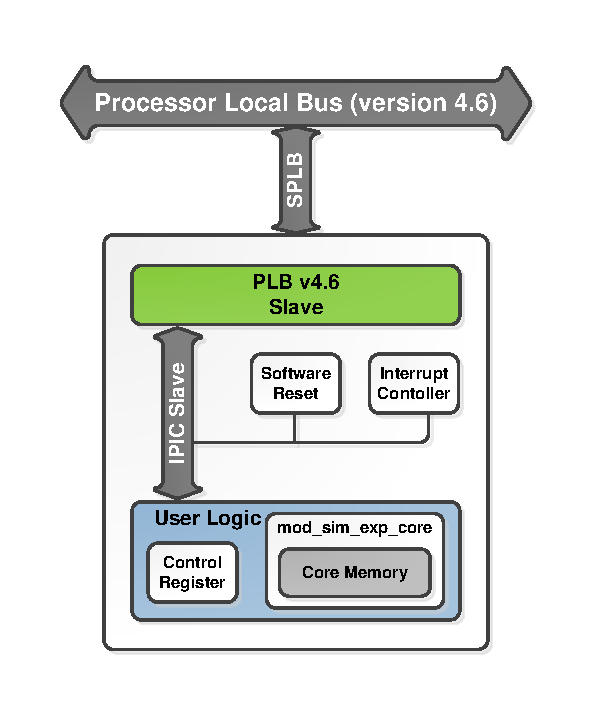
\includegraphics[trim=1.2cm 1.2cm 1.2cm 1.2cm, width=7cm]{pictures/plb_interface.pdf}
\caption{PLB IP core structure}
\label{PLBstructure}
\end{figure}

\newpage
\section{Parameters}
This section describes the parameters used to configure the core, only the relevant parameters are discussed. PLB
specific parameters are left to the user to configure. The IP core specific parameters and their respective use are
listed in the table below.
\begin{center}
	\begin{tabular}{|l|p{6.5cm}|c|l|}
		\hline
		\rowcolor{Gray}
		\textbf{Name} & \textbf{Description} & \textbf{VHDL Type} &\textbf{Default Value} \bigstrut\\
		\hline
		\multicolumn{4}{|l|}{\textit{\textbf{Memory configuration}}} \\		
		\hline
		\verb|C_FIFO_AW| & address width of the generic FIFO pointers, FIFO size is equal to $2^{C\_FIFO\_AW} $. & integer & 7 \bigstrut\\
						 & only	applicable if \verb|C_MEM_STYLE| = \verb|"generic"| or \verb|"asym"|  & & \\
		\hline
		\verb|C_MEM_STYLE| & the memory structure to use for the RAM, choice between 3 options: & string & \verb|"generic"| \bigstrut\\
							& \verb|"xil_prim"| : use xilinx primitives & & \\
      						& \verb|"generic"| : use general 32-bit RAMs & & \\
      						& \verb|"asym"| : use asymmetric RAMs & & \\
      						& (For more information see \ref{subsec:RAM_and_FIFO}) & & \bigstrut[b] \\
		\hline
		\verb|C_FPGA_MAN| & device manufacturer: & string & \verb|"xilinx"| \\
						& \verb|"xilinx"| or \verb|"altera"| &  &  \bigstrut\\
		\hline
		\verb|C_BASEADDR| & base address for the IP core's memory space & std\_logic\_vector & X"FFFFFFFF" \bigstrut\\
		\hline
		\verb|C_HIGHADDR| & high address for the IP core's memory space & std\_logic\_vector & X"00000000" \bigstrut\\
		\hline
		\verb|C_M_BASEADDR| & base address for the modulus memory space & std\_logic\_vector & X"FFFFFFFF" \bigstrut\\
		\hline
		\verb|C_M_HIGHADDR| & high address for the modulus memory space & std\_logic\_vector & X"00000000" \bigstrut\\
		\hline
		\verb|C_OP0_BASEADDR| & base address for the operand 0 memory space & std\_logic\_vector & X"FFFFFFFF" \bigstrut\\
		\hline
		\verb|C_OP0_HIGHADDR| & high address for the operand 0 memory space & std\_logic\_vector & X"00000000" \bigstrut\\
		\hline
		\verb|C_OP1_BASEADDR| & base address for the operand 1 memory space & std\_logic\_vector & X"FFFFFFFF" \bigstrut\\
		\hline
		\verb|C_OP1_HIGHADDR| & high address for the operand 1 memory space & std\_logic\_vector & X"00000000" \bigstrut\\
		\hline
		\verb|C_OP2_BASEADDR| & base address for the operand 2 memory space & std\_logic\_vector & X"FFFFFFFF" \bigstrut\\
		\hline
		\verb|C_OP2_HIGHADDR| & high address for the operand 2 memory space & std\_logic\_vector & X"00000000" \bigstrut\\
		\hline
		\verb|C_OP3_BASEADDR| & base address for the operand 3 memory space & std\_logic\_vector & X"FFFFFFFF" \bigstrut\\
		\hline
		\verb|C_OP3_HIGHADDR| & high address for the operand 3 memory space & std\_logic\_vector & X"00000000" \bigstrut\\
		\hline
		\verb|C_FIFO_BASEADDR| & base address for the FIFO memory space & std\_logic\_vector & X"FFFFFFFF" \bigstrut\\
		\hline
		\verb|C_FIFO_HIGHADDR| & high address for the FIFO memory space & std\_logic\_vector & X"00000000" \bigstrut\\
		\hline
		\multicolumn{4}{|l|}{\textit{\textbf{Multiplier configuration}}} \\
		\hline
		\verb|C_NR_BITS_TOTAL| & total width of the multiplier in bits & integer & 1536\bigstrut\\
		\hline
		\verb|C_NR_STAGES_TOTAL| & total number of stages in the pipeline & integer & 96\bigstrut\\
		\hline
		\verb|C_NR_STAGES_LOW| & number of lower stages in the pipeline, defines the bit-width of the lower pipeline part & integer & 32 \bigstrut\\
		\hline
		\verb|C_SPLIT_PIPELINE| & option to split the pipeline in 2 parts & boolean & true \bigstrut\\
		\hline
	\end{tabular}%
\end{center}
%\newline 

The complete IP core's memory space can be controlled. As can be seen, the operand, modulus and FIFO memory space can be
chosen separately from the IP core's memory space which hold the registers for control, software reset and interrupt
control. The core's memory space must have a minimum width of 1K byte for all registers to be accessible. For the FIFO
memory space, a minimum width of 4 byte is needed, since the FIFO is only 32 bit wide. The memory space width for the
operands and the modulus need a minimum width equal to the total multiplier width.\\

There are 4 parameters to configure the multiplier. These values define the width of the multiplier operands and the
number of pipeline stages. If \verb|C_SPLIT_PIPELINE| is false, only operands with a width of\\\verb|C_NR_BITS_TOTAL| are
valid. Else if \verb|C_SPLIT_PIPELINE| is true, 3 operand widths can be supported:
\begin{itemize}
  \item the length of the full pipeline ($C\_NR\_BITS\_TOTAL$)
  \item the length of the lower pipeline ($\frac{C\_NR\_BITS\_TOTAL}{C\_NR\_STAGES\_TOTAL} \cdot C\_NR\_STAGES\_LOW $)
  \item the length of the higher pipeline ($\frac{C\_NR\_BITS\_TOTAL}{C\_NR\_STAGES\_TOTAL} \cdot (C\_NR\_STAGES\_TOTAL - C\_NR\_STAGES\_LOW$)
\end{itemize}

\section{IO ports}
\begin{tabular}{|l|c|c|l|}
	\hline
	\rowcolor{Gray}
	\textbf{Port} & \textbf{Width} & \textbf{Direction} & \textbf{Description} \\
	\hline
	\multicolumn{4}{|l|}{\textit{\textbf{PLB bus connections}}} \\
	\hline
	\verb|SPLB_Clk| & 1     & in & see note 1 \\
	\hline
	\verb|SPLB_Rst| & 1     & in & see note 1 \\
	\hline
	\verb|PLB_ABus| & 32    & in & see note 1 \\
	\hline
	\verb|PLB_PAValid| & 1     & in & see note 1 \\
	\hline
	\verb|PLB_masterID| & 3     & in & see note 1 \\
	\hline
	\verb|PLB_RNW| & 1     & in & see note 1 \\
	\hline
	\verb|PLB_BE| & 4     & in & see note 1 \\
	\hline
	\verb|PLB_size| & 4     & in & see note 1 \\
	\hline
	\verb|PLB_type| & 3     & in & see note 1 \\
	\hline
	\verb|PLB_wrDBus| & 32    & in & see note 1 \\
	\hline
	\verb|Sl_addrAck| & 1     & out & see note 1 \\
	\hline
	\verb|Sl_SSize| & 2     & out & see note 1 \\
	\hline
	\verb|Sl_wait| & 1     & out & see note 1 \\
	\hline
	\verb|Sl_rearbitrate| & 1     & out & see note 1 \\
	\hline
	\verb|Sl_wrDack| & 1     & out & see note 1 \\
	\hline
	\verb|Sl_wrComp| & 1     & out & see note 1 \\
	\hline
	\verb|Sl_rdBus| & 32    & out & see note 1 \\
	\hline
	\verb|Sl_MBusy| & 8     & out & see note 1 \\
	\hline
	\verb|Sl_MWrErr| & 8     & out & see note 1 \\
	\hline
	\verb|Sl_MRdErr| & 8     & out & see note 1 \\
	\hline
	\multicolumn{4}{|l|}{\textit{\textbf{unused PLB signals}}} \\
	\hline
	\verb|PLB_UABus| & 32    & in & see note 1 \\
	\hline
	\verb|PLB_SAValid| & 1     & in & see note 1 \\
	\hline
	\verb|PLB_rdPrim| & 1     & in & see note 1 \\
	\hline
	\verb|PLB_wrPrim| & 1     & in & see note 1 \\
	\hline
	\verb|PLB_abort| & 1     & in & see note 1 \\
	\hline
	\verb|PLB_busLock| & 1     & in & see note 1 \\
	\hline
	\verb|PLB_MSize| & 2     & in & see note 1 \\
	\hline
	\verb|PLB_TAttribute| & 16    & in & see note 1 \\
	\hline
	\verb|PLB_lockerr| & 1     & in & see note 1 \\
	\hline
	\verb|PLB_wrBurst| & 1     & in & see note 1 \\
	\hline
	\verb|PLB_rdBurst| & 1     & in & see note 1 \\
	\hline
	\verb|PLB_wrPendReq| & 1     & in & see note 1 \\
	\hline
	\verb|PLB_rdPendReq| & 1     & in & see note 1 \\
	\hline
	\verb|PLB_rdPendPri| & 2     & in & see note 1 \\
	\hline
	\verb|PLB_wrPendPri| & 2     & in & see note 1 \\
	\hline
	\verb|PLB_reqPri| & 2     & in & see note 1 \\
	\hline
	\verb|Sl_wrBTerm| & 1     & out & see note 1 \\
	\hline
	\verb|Sl_rdWdAddr| & 4     & out & see note 1 \\
	\hline
	\verb|Sl_rdBTerm| & 1     & out & see note 1 \\
	\hline
	\verb|Sl_MIRQ| & 8     & out & see note 1 \\
	\hline
	\multicolumn{4}{|l|}{\textit{\textbf{Core signals}}} \\
	\hline
	\verb|IP2INTC_Irpt| & 1     & out   & core interrupt signal \\
	\hline
	\verb|calc_time| & 1     & out   & is high when core is performing a multiplication, for monitoring \\
	\hline
\end{tabular}%
\newline \newline
\textbf{Note 1:} The function and timing of this signal is defined in the IBM\textsuperscript{\textregistered} 128-Bit Processor Local Bus Architecture Specification
Version 4.6.

\section{Registers}
This section specifies the IP core internal registers as seen from the software. These registers allow to control and
configure the modular exponentiation core and to read out its state. All addresses given in this table are relative to the
IP core's base address.\\
\newline
% Table generated by Excel2LaTeX
\begin{tabular}{|l|c|c|c|l|}
\hline
\rowcolor{Gray}
\textbf{Name} & \textbf{Width} & \textbf{Address} & \textbf{Access} & \textbf{Description} \bigstrut\\
\hline
control register 		& 32 & 0x0000 & RW 	& multiplier core control signals and \bigstrut[t]\\
						&	&		&		& interrupt flags register\bigstrut[b]\\
\hline
software reset			& 32 & 0x0100 & W 	& soft reset for the IP core  \bigstrut\\
\hline
\multicolumn{5}{|l|}{\textbf{\textit{Interrupt controller registers}}} \bigstrut\\
\hline
global interrupt enable register 	& 32 & 0x021C & RW & global interrupt enable for the IP core \bigstrut[t]\\
interrupt status register			& 32 & 0x0220 &	R  & register for interrupt status flags\\
interrupt enable register			& 32 & 0x0228 & RW & register to enable individual IP core interrupts \bigstrut[b]\\
\hline
\end{tabular}%

\newpage
\subsection{Control register (offset = 0x0000)}
This registers holds the control inputs to the multiplier core and the interrupt flags.\\
\begin{figure}[H]
\centering
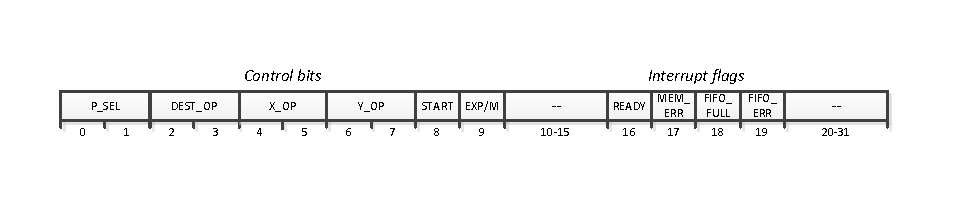
\includegraphics[trim=1.2cm 1.2cm 1.2cm 1.2cm, width=15cm]{pictures/plb_control_reg.pdf}
\caption{control register}
\end{figure}


\begin{tabular}{ll}
bits 0-1 	& P\_SEL : selects which pipeline part to be active\\
 			& $\bullet$  "01" lower pipeline part\\
 			& $\bullet$  "10" higher pipeline part\\
 			& $\bullet$  "11" full pipeline\\
 			& $\bullet$  "00" invalid selection\\
 			&\\
bits 2-3 	& DEST\_OP : selects the operand (0-3) to store the result in for a single\\
 			& Montgomery multiplication\footnotemark\\
 			&\\
bits 4-5 	& X\_OP : selects the x operand (0-3) for a single Montgomery multiplication\footnotemark[\value{footnote}]\\
			&\\
bits 6-7 	& Y\_OP : selects the y operand (0-3) for a single Montgomery multiplication\footnotemark[\value{footnote}]\\
			&\\
bit 8 		& START : starts the multiplication/exponentiation\\
			&\\
bit 9 		& EXP/M : selects the operating mode\\
 			& $\bullet$  "0" single Montgomery multiplications\\
 			& $\bullet$  "1" simultaneous exponentiations\\
 			&\\
bits 10-15	& unimplemented\\
			&\\
bit 16		& READY : ready flag, "1" when multiplication is done\\
			& must be cleared in software\\
			&\\
bit 17		& MEM\_ERR : memory collision error flag, "1" when write error occurred\\
			& must be cleared in software\\
			&\\
bit 18		& FIFO\_FULL : FIFO full error flag, "1" when FIFO is full\\
			& must be cleared in software\\
			&\\
bit 19		& FIFO\_ERR : FIFO write/push error flag, "1" when push error occurred\\
			& must be cleared in software\\
			&\\
bits 20-31	& unimplemented\\
			&\\
\end{tabular}
\newline
\newline
\footnotetext{when the core is running in exponentiation mode, the parameters DEST\_OP, X\_OP and Y\_OP have no effect.}

\newpage
\subsection{Software reset register (offset = 0x0100)}
This is a register with write only access, and provides the possibility to reset the IP core from software by writing
0x0000000A to this address. The reset affects the full IP core, thus resetting the control register, interrupt controller,
the multiplier pipeline, FIFO and control logic of the core.

\subsection{Global interrupt enable register (offset = 0x021C)}
This register contains a single defined bit in the high-order position. The GIE bit enables or disables all interrupts
form the IP core.\\
\begin{figure}[H]
\centering
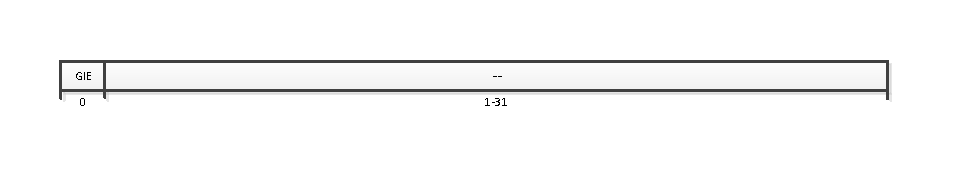
\includegraphics[trim=1.2cm 1.2cm 1.2cm 1.2cm, width=15cm]{pictures/plb_gie_reg.pdf}
\caption{Global interrupt enable register}
\end{figure}

\begin{tabular}{ll}
bit 0 		& GIE : Global interrupt enable\\
 			& $\bullet$  "0" disables all core interrupts\\
 			& $\bullet$  "1" enables all core interrupts\\
 			&\\
bits 1-31	& unimplemented\\
			&\\
\end{tabular}

\subsection{Interrupt status register (offset = 0x0220)}
Read-only register that contains the status of the core interrupts. Currently there is only one common interrupt from
the core that is asserted when a multiplication/exponentiation is done, FIFO is full, on FIFO push error or memory write
collision.\\
\begin{figure}[H]
\centering
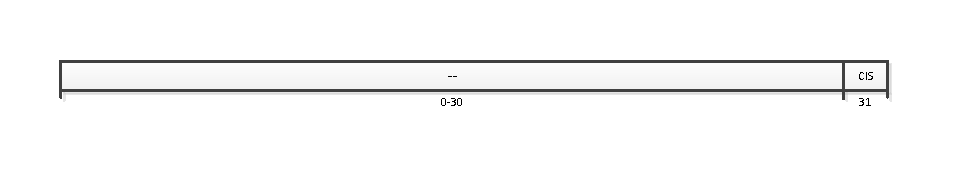
\includegraphics[trim=1.2cm 1.2cm 1.2cm 1.2cm, width=15cm]{pictures/plb_is_reg.pdf}
\caption{Interrupt status register}
\end{figure}

\begin{tabular}{ll}
bits 0-30	& unimplemented\\
			&\\
bit 31 		& CIS : Core interrupt status\\
 			& is high when interrupt is requested from core\\
 			&\\
\end{tabular}

\subsection{interrupt enable register (offset = 0x0228)}
This register contains the interrupt enable bits for the respective interrupt bits of the interrupt status register.\\
\begin{figure}[H]
\centering
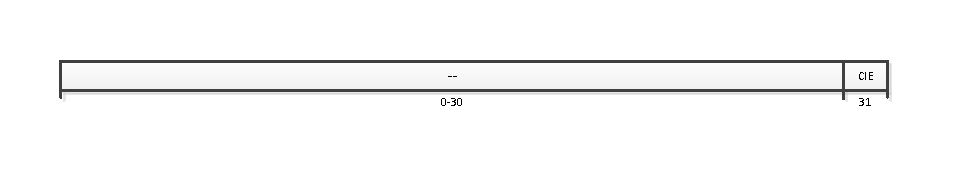
\includegraphics[trim=1.2cm 1.2cm 1.2cm 1.2cm, width=15cm]{pictures/plb_ie_reg.pdf}
\caption{Interrupt enable register}
\end{figure}
\begin{tabular}{ll}
bits 0-30	& unimplemented\\
			&\\
bit 31 		& CIE : Core interrupt enable\\
 			& $\bullet$  "0" disable core interrupt\\
 			& $\bullet$  "1" enable core interrupt\\
 			&\\
\end{tabular}

\section{Interfacing the core's RAM}
Special attention must be taken when writing data to the operands and modulus. The least significant bit of the data has be on the lowest
address and the most significant bit on the highest address. A write to the RAM has to happen 1 word at a time, byte writes are not
supported due to the structure of the RAM.

\section{Handling interrupts}
When the embedded processor receives an interrupt signal from this core, it is up to the controlling software to
determine the source of the interrupt by reading out the interrupt flag of the control register.